\documentclass{article}
\usepackage[utf8]{inputenc}
\usepackage{amsmath}
\usepackage{amssymb}
\usepackage{mathtools}
\usepackage{mcode}
\usepackage{graphicx}

\graphicspath{{Images/}}


\setlength{\oddsidemargin}{0in}
\setlength{\textwidth}{6.5in}
\setlength{\topmargin}{-.55in}
\setlength{\textheight}{9in}
\pagestyle{empty}


\title{Scientific Computation Homework 6}
\author{Michael Nameika}
\date{October 2022}

\begin{document}

\maketitle

\section*{Exercise 9.1}
Consider the following method for solving the heat equation $u_t = u_{xx}$:
\[U_i^{n+2} = U_i^n + \frac{2k}{h^2}(U^{n+1}_{i-1} - 2U_i^{n+1} + U_{i+1}^{n+1}).\]
\begin{itemize}
    \item[(a)] Determine the order of accuracy of this method (in both space and time).
    \newline
    
    To begin, let us rearrange the method into the following form:
    \[\frac{U_i^{n+2} - U_i^n}{2k} = \frac{U^{n+1}_{i-1} - 2U_i^{n+1} + U_{i+1}^{n+1}}{h^2}\]
    Writing the above equation in exact form, we have
    \[\frac{u_i^{n+2} - u_i^n}{2k} = \frac{u^{n+1}_{i-1} - 2u_i^{n+1} + u_{i+1}^{n+1}}{h^2}\]
    Let us begin by Taylor expanding the left hand side. Notice
    \begin{align*}
        u_i^{n+2} = u_i^n + 2k \frac{\partial u_i^n}{\partial t} + 2k^2\frac{\partial^2 u_i^n}{\partial t^2} + \frac{4}{3}k^3\frac{\partial^3u_i^n}{\partial t^3} + \mathcal{O}(k^4) \\
    \end{align*}
    Then
    \begin{align*}
        \frac{u_i^{n+2} - u_i^n}{2k} &= \frac{\partial u_i^n}{\partial t} + k\frac{\partial^2u_i^n}{\partial t^2} + \frac{2}{3}k^2\frac{\partial^3u_i^n}{\partial t^3} + \mathcal{O}(k^4) \\
    \end{align*}
    Now let us Taylor expand the right hand side:
    \begin{align*}
        u_{i-1}^{n+1} &= u^{n+1}_i - h\frac{\partial u^{n+1}_i}{\partial x} + \frac{h^2}{2}\frac{\partial^2u_i^{n+1}}{\partial x^2} - \frac{h^3}{3!}\frac{\partial^3u_i^{n+1}}{\partial x^3} + \frac{h^4}{4!}\frac{\partial^4u_i^{n+1}}{\partial x^4} - \frac{h^5}{5!}\frac{\partial^5u_i^{n+1}}{\partial x^5} + \mathcal{O}(h^6) \\
        u_{i+1}^{n+1} &= u^{n+1}_i + h\frac{\partial u^{n+1}_i}{\partial x} + \frac{h^2}{2}\frac{\partial^2u_i^{n+1}}{\partial x^2} + \frac{h^3}{3!}\frac{\partial^3u_i^{n+1}}{\partial x^3} + \frac{h^4}{4!}\frac{\partial^4u_i^{n+1}}{\partial x^4} + \frac{h^5}{5!}\frac{\partial^5u_i^{n+1}}{\partial x^5} + \mathcal{O}(h^6) \\
    \end{align*}
    Then
    \begin{align*}
        \frac{u_{i-1}^{n+1} - 2u_i^{n+1} + u_{i+1}^{n+1}}{h^2} &= \frac{\partial^2 u_i^{n+1}}{\partial x^2} + \frac{2}{4!}h^2\frac{\partial^4 u_i^{n+1}}{\partial x^4} + \mathcal{O}(h^4) \\
    \end{align*}
    And so our local truncation error takes the following form:
    \begin{align*}
        \tau(x,t) &= \frac{\partial u_i^n}{\partial t} + k\frac{\partial^2 u_i^n}{\partial t^2} + \frac{2}{3}k^2\frac{\partial^3u_i^n}{\partial t^3} - \frac{\partial^2 u_i^{n+1}}{\partial x^2} + \mathcal{O}(h^2) + \mathcal{O}(k^3) \\
    \end{align*}
    To simplify our local truncation error any further, we must Taylor expand $u_i^{n+1}$:
    \[u_i^{n+1} = u_i^n + k\frac{\partial u_i^n}{\partial t} + \frac{k^2}{2}\frac{\partial^2u_i^n}{\partial t^2} + \frac{k^3}{3!}\frac{\partial^3u^n_i}{\partial t^3} + \mathcal{O}(k^4)\]
    Using this in our equation for the local truncation error leads us to
    \begin{align*}
        \tau(x,t) &= \frac{\partial u_i^n}{\partial t} + k\frac{\partial^2 u_i^n}{\partial t^2} + \frac{2}{3}k^2\frac{\partial^3u_i^n}{\partial t^3} - \frac{\partial^2u^n_i}{\partial x^2} - k\frac{\partial^2}{\partial x^2}\left(\frac{\partial u_i^n}{\partial t}\right) - \frac{k^2}{2}\frac{\partial^2}{\partial x^2}\left(\frac{\partial^2u_i^n}{\partial t^2}\right) - \frac{k^3}{3!}\frac{\partial^2}{\partial x^2}\left(\frac{\partial^3u_i^n}{\partial t^3}\right) + \mathcal{O}(k^4 + h^2) \\
    \end{align*}
    From our differential equation, we have $\frac{\partial u_i^n}{\partial t} = \frac{\partial^2u_i^n}{\partial x^2}$, so our local truncation error becomes
    \begin{align*}
        \tau(x,t) &= \frac{\partial u_i^n}{\partial t} + k\frac{\partial^2 u_i^n}{\partial t^2} + \frac{2}{3}k^2\frac{\partial^3u_i^n}{\partial t^3} - \frac{\partial u^n_i}{\partial t} - k\frac{\partial^2u_i^n}{\partial t^2} - \frac{k^2}{2}\frac{\partial^3u_i^n}{\partial t^2} - \frac{k^3}{3!}\frac{\partial^4 u_i^n}{\partial t^4} + \mathcal{O}(k^4 + h^2) \\
        &= \frac{k^2}{6}\frac{\partial^3u_i^n}{\partial t^3} + \mathcal{O}(k^3 + h^2) \\
    \end{align*}
    So 
    \[\tau(x,t) = \mathcal{O}(k^2 + h^2)\]
    That is, this method is second order accurate in both space and time.
    \newline\newline
    \item[(b)] Suppose we take $k = \alpha h^2$ for some fixed $\alpha > 0$ and refine the grid. For what values of $\alpha$ (if any) will this method be Lax-Richtmyer stable and hence convergent?
    \newline
    \textbf{Hint}: Consider the MOL interpretation and the stability region of the time-discretization being used.
    \newline
    We require $|\lambda| \leq 1$ for stability. Additionally, we have $|1 - k/(2h^2)\lambda| \leq 1$ which leads us to 
    \begin{align*}
        \frac{k}{2h^2} &\leq 2 \\
        \alpha &\leq 4 \\
    \end{align*}
    
    
    
    \item[(c)] Is this a useful method?
    \newline
    It's second order accurate in both space and time, so why not?
    
\end{itemize}

\section*{Exercise 9.2}
\begin{itemize}
    \item[(a)] The m-file  \mcode{heat_CN.m} solves the heat equation $u_t = \kappa u_{xx}$ using the Crank-Nicolson method. Run this code, and by changing the number of grid points, confirm that it is second-order accurate. (Observe how the error at some fixed time such as $T = 1$ behaves as $k$ and $h$ go to zero with a fixed relation between $k$ and $h$, such as $k = 4h$.)
    \newline
    You might want to use the function \mcode{error_table.m} to print out this table and estimate the order of accuracy, and \mcode{error_loglog.m} to produce a log-log plot of the error vs. $h$. See \mcode{bvp_2.m} for an example of how these are used
    \newline\newline
    Running \mcode{heat_CN.m} for decreasing values of $h$, we find the following:
    \begin{center}
        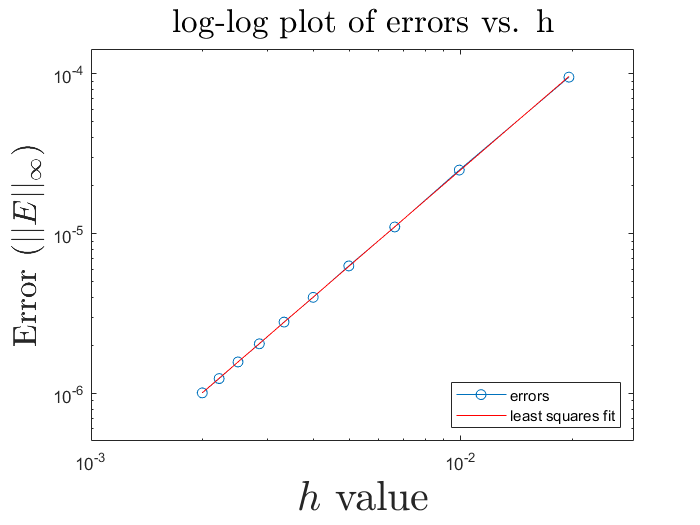
\includegraphics[scale = 0.4]{crankNicolsonerrGraph.png}
        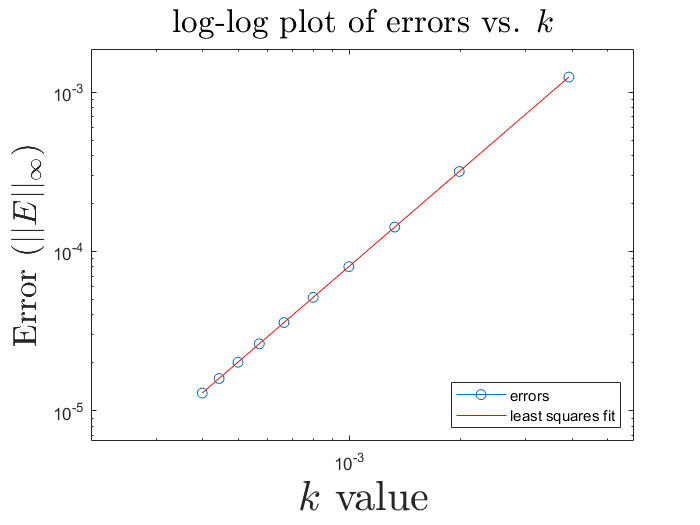
\includegraphics[scale = 0.4]{cnorderk.png}
        \newline
        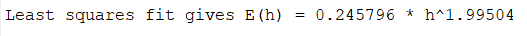
\includegraphics[scale = 0.55]{CNerrororder.PNG}
        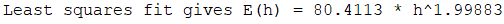
\includegraphics[scale = 0.55]{cnerrork.PNG}
    \end{center}
    Which shows us that the Crank-Nicolson method is second order accurate in both space and time.
    
    \item[(b)] Modify \mcode{heat_CN.m} to produce a new m-file \mcode{heat_trbdf2.m} that implements the TR-BDF2 method on the same problem. Test it to confirm that it is also second order accurate. Explain how you determined the proper boundary conditions in each stage of this Runge-Kutta method.
    \newline\newline
    Recall that the TR-BDF2 method has the following form:
    \begin{align*}
        U^* &= U^n + \frac{\Delta t}{4}(f(U^n) + f(U^*))\\
        U^{n+1} &= \frac{1}{3}(4U^* - U^n + f(U^{n+1})) \\
    \end{align*}
    Applying this method to $u_{tt} = \kappa u_{xx}$, we will find the following for $U^*$:
    \begin{align*}
        U^* &= U^n + \frac{\Delta t}{2}\left(\frac{f(U^n) + f(U^*)}{2}\right) \\
    \end{align*}
    Which shows that $U^*$ is a half step increment in time, and using the method of lines (MOL) to rewrite as discrete system, we have
    \begin{align*}
        u^*_i &= u^n_i +  \kappa\frac{\Delta t}{2\Delta x^2}\left(\frac{u_{i+1}^n - 2u_i^n + u_{i-1}^n}{2} + \frac{u_{i+1}^{n+1/2} - 2u_i^{n + 1/2} + u_{i-1}^{n+1/2}}{2}\right) \\
    \end{align*}
    and for $i = 1$,
    \begin{align*}
        u^*_1 &= u^n_1 + \kappa \frac{\Delta t}{2\Delta x^2}\left(\frac{u_2^n - 2u_i^n + u_0^n}{2} + \frac{u^{n+1/2}_2 - 2u_1^{n+1/2} + u_0^{n+1/2}}{2} \right)\\
    \end{align*}
    Writing this step in matrix notation, we have
    \begin{align*}
        A^*U^* = A_RU^n + G^n_1\\
    \end{align*}
    where 
    \begin{align*}
        A^* &= \begin{bmatrix}
         1 + 2r & -r & & & \\
         -r & 1 + 2r & -r & & \\
           & \ddots & \ddots & \ddots & \\
           & & -r & 1 + 2r & -r \\
           & & & -r & 1 + 2r \\
        \end{bmatrix} \\
        A_R &= \begin{bmatrix}
         1 - 2r & r & & & \\
         r & 1 - 2r & r & & \\
           & \ddots & \ddots & \ddots & \\
           & & r & 1 - 2r & r \\
           & & & r & 1 - 2r \\
        \end{bmatrix}\\
        G^n_1 &= \begin{bmatrix}
            g_0^n + g_0^{n+1/2} \\
            0\\
            \vdots\\
            0\\
            g_1^n + g_1^{n+1/2}\\
        \end{bmatrix}
    \end{align*}
    and
    \[r = \frac{\kappa\Delta t}{4\Delta x^2}\]
    Now, to for the implicit step, we can see, similar to the work above, that 
    \begin{align*}
        A_LU^{n+1} &= \frac{4}{3}U^* -\frac{1}{3}U^n\\
    \end{align*}
    where 
    \begin{align*}
        A_L &= \begin{bmatrix}
            1 + 4/3r & -4/3r & & & \\
            -4/3r & 1 + 4/3r & -4/3r & & \\
            & \ddots & \ddots & \ddots & \\
            & & -4/3r & 1 + 4/3r & -4/3r \\
            & & & -4/3r & 1 + 4/3r \\
        \end{bmatrix}
    \end{align*}
    Implementing this method by modifying \mcode{heat_CN.m} (see attached \mcode{.m} file), we find the following for the order of accuracy:
    \begin{center}
        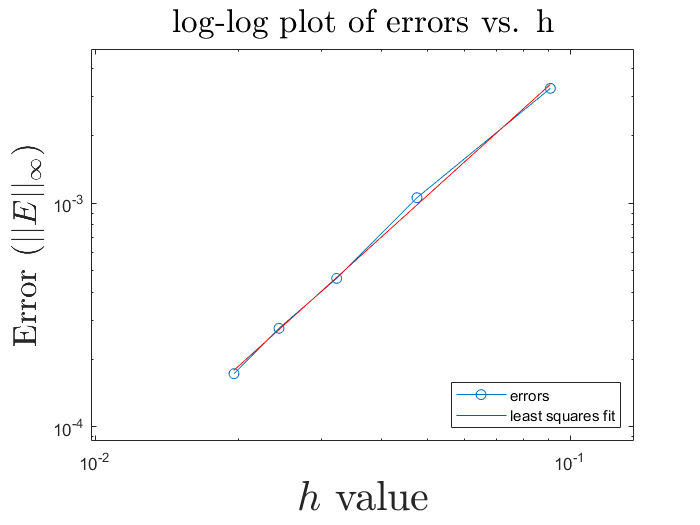
\includegraphics[scale= 0.4]{trbdferrGauss.png}
        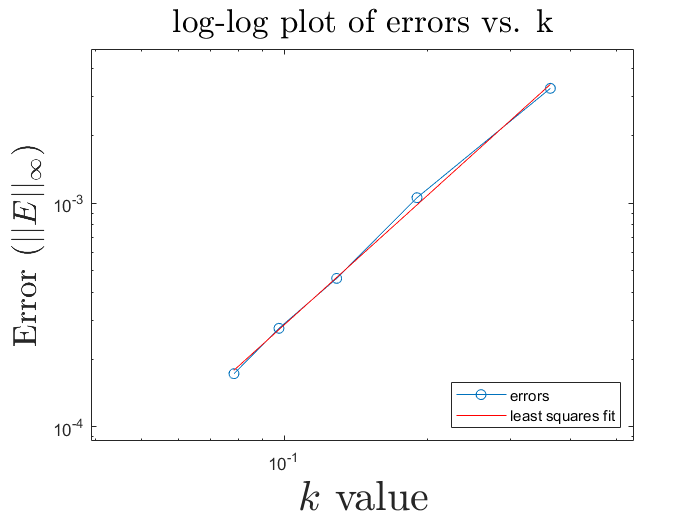
\includegraphics[scale = 0.4]{kerrTRBDF2Gauss.png}
        \newline
        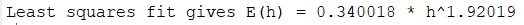
\includegraphics[scale = 0.6]{horderTRBDF2Gauss.PNG}
        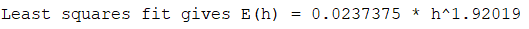
\includegraphics[scale = 0.6]{kerrorderTRBDF2Gauss.PNG}
    \end{center}
    So we can see the TR-BDF2 method is second order accurate in both space and time.
    
    \item[(c)] Modify \mcode{heat_CN.m} to produce a new m-file \mcode{heat_FE.m} that implements the forward Euler explicit method on the same problem. Test it to confirm that it is $\mathcal{O}(h^2)$ accurate as $h \to 0$ provided when $k = 24h^2$ is used, which is within the stability limit for $\kappa = 0.02$. Note how many more time steps are required than with Crank-Nicolson or TR-BDF2, especially on finer grids.
    \newline\newline
    Modifying \mcode{heat_CN.m} to implement the Forward-Euler method, and using $k = 24h^2$, we find the following for smaller values of $h$:
    \begin{center}
        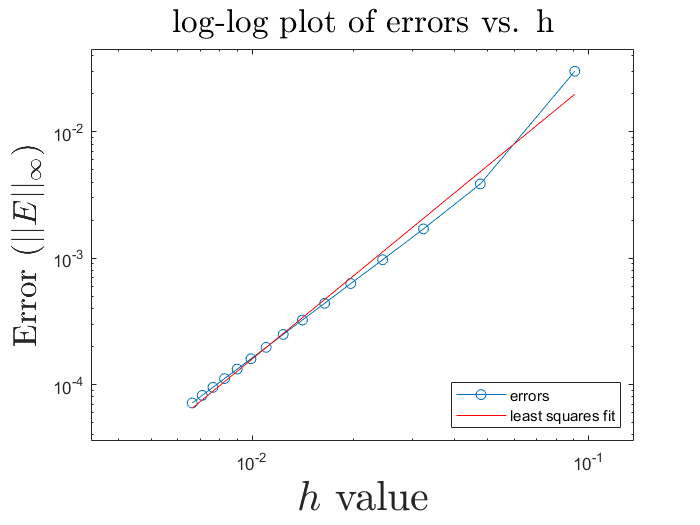
\includegraphics[scale = 0.6]{loglogerrorforFE.png}
        \newline
        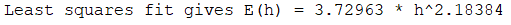
\includegraphics[scale = 0.8]{FEorder.PNG}
    \end{center}
    which shows us that the method is approximately second order accurate in space.
    
    \item[(d)] Test \mcode{heat_FE.m} with $k = 26h^2$, for which it should be unstable. Note that the instability does not become apparent until about time 1.6 for the parameter values $\kappa = 0.02$, $m = 39$, $\beta = 150$. Explain why the instability takes several undred time steps to appear, and why it appears as a sawtooth oscillation.
    \newline\newline
    Changing $k = 26h^2$, we find the following plot for the solutions in time using the Forward-Euler method:
    \begin{center}
        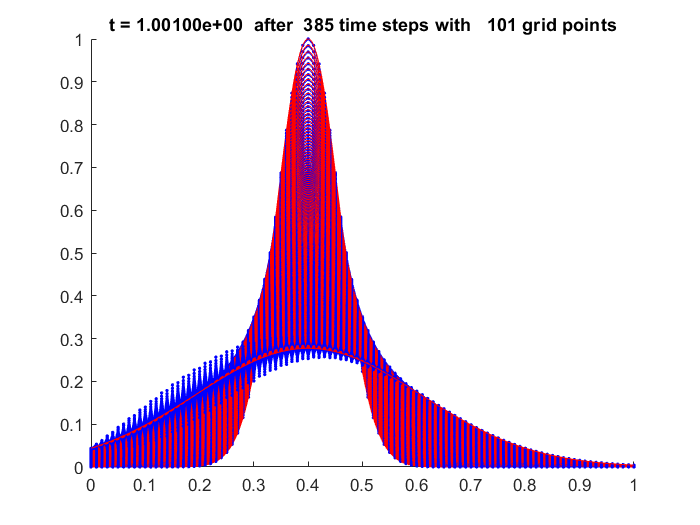
\includegraphics[scale = 0.6]{FE26h2.png}
    \end{center}
    Notice how the solutions at later time steps have this 'sawtooth' instability. Curiously, using $m=39$ did not show this instability and the instabilities did not show up until about $t = 0.9$.
    
\end{itemize}

\section*{Exercise 9.3}
\begin{itemize}
    \item[(a)] Modify \mcode{heat_CN.m} to solve the heat equation for $-1 \leq x \leq 1$ with step function initial data
    \[u(x,0) = \begin{cases}
        1 &\text{if } x < 0 \\
        0 &\text{if } x \geq 0.\\
    \end{cases}\]
    With appropriate Dirichlet boundary conditions, the exact solution is
    \[u(x,t) = \frac{1}{2}\text{erfc}(x/\sqrt{4\kappa t}),\]
    where erfc is the complementary error function
    \[\text{erfc}(x) = \frac{2}{\sqrt{\pi}}\int_x^{\infty}e^{-z^2}dz.\]
    \begin{itemize}
        \item[(i)] Test this routine $m = 39$ and $k = 4h$. Note that there is an initial rapid transient decay of the high wave numbers that is not captured well with this size time step.
        \newline\newline
        Modifying the \mcode{heat_CN.m} (see attached code), we find the following for $m = 39$ and $k = 4h$:
        
            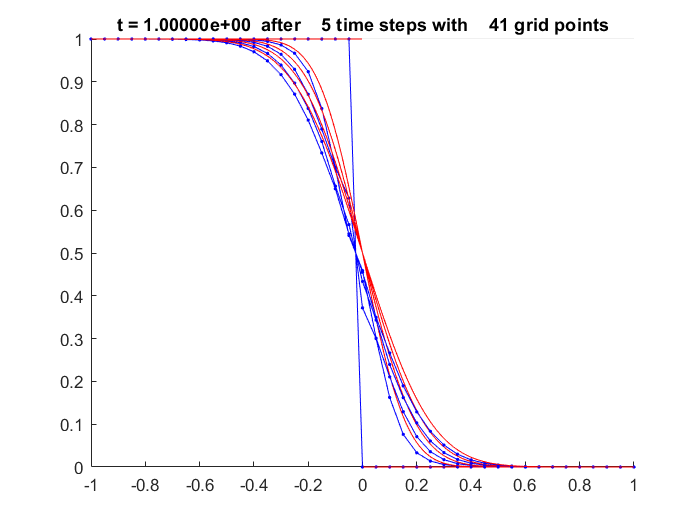
\includegraphics[scale = 0.6]{erf39.png}
            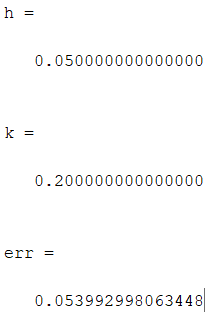
\includegraphics[scale = 0.7]{err39.PNG}
        
        
        
        
        \item[(ii)] How small do you need to take the time step to get reasonable results? For a suitably small time step, explain why you get much better results by using $m=38$ than $m=39$. What is the observed order of accuracy as $k \to 0$ when $k = \alpha h$ with $\alpha$ suitably small and $m$ even?
        \newline\newline
        Presumably, it would be reasonable to assume that $k \leq 1/2$ to get reasonable results since, if $k > 1/2$, we would have only one time step, which would mean only the initial data will be approximated. 
        Having $k \leq 1/2$ will give us at least one approximation that will allow us to see the continuous solution. 
        
        We get much better results by using $m = 38$ rather than $m = 39$ since for odd values of $m$, we will be including the midpoint discontinuity in the approximation, which will lead to the approximation "undershooting" the actual approximation.
        \newline
        Running the program for $\alpha = 1/10$, we find the following for the order of accuracy in $k$:
        \begin{center}
            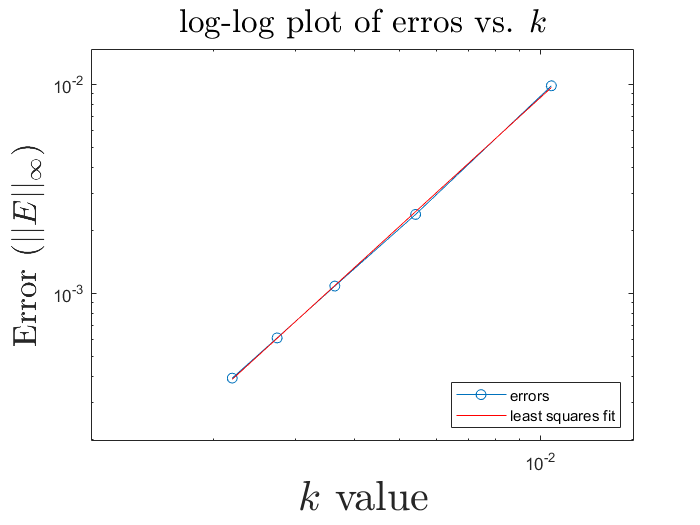
\includegraphics[scale = 0.6]{93errork.png}
            \newline
            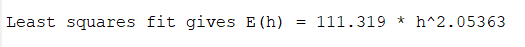
\includegraphics[scale = 0.8]{orderink.PNG}
        \end{center}
        
    \end{itemize}
    \item[(b)] Modify \mcode{heat_trbdf2.m} (see Exercise 9.2) to solve the heat equation for $-1 \leq x \leq 1$ with step function initial data as above. Test this routine using $k = 4h$ and estimate the order of accuracy as $k \to 0$ with $m$ even. Why does the TR-BDF2 method work better than Crank-Nicolson?
    \newline\newline
    Modifying the \mcode{heat_trbdf2.m} we used earlier in the assignment, we find the following for an even number of spacial points:
    \begin{center}
        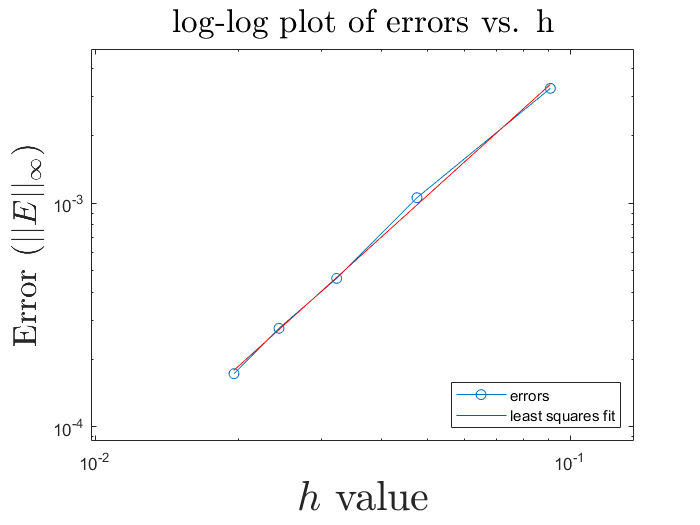
\includegraphics[scale = 0.4]{trbdferrGauss.png}
        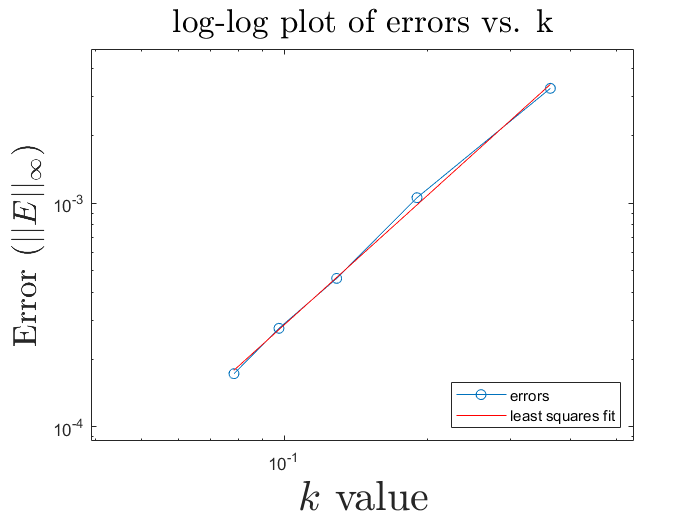
\includegraphics[scale = 0.4]{kerrTRBDF2Gauss.png}
        \newline
        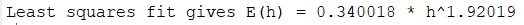
\includegraphics[scale =0.6]{horderTRBDF2Gauss.PNG} 
        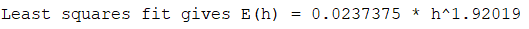
\includegraphics[scale =0.6]{kerrorderTRBDF2Gauss.PNG} 
    \end{center}
    and for an odd number of spacial points:
    \begin{center}
        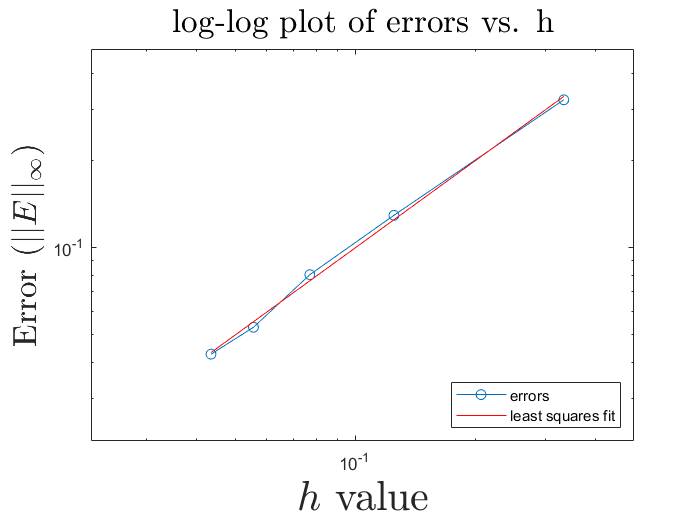
\includegraphics[scale = 0.4]{trbdf2errorh.png}
        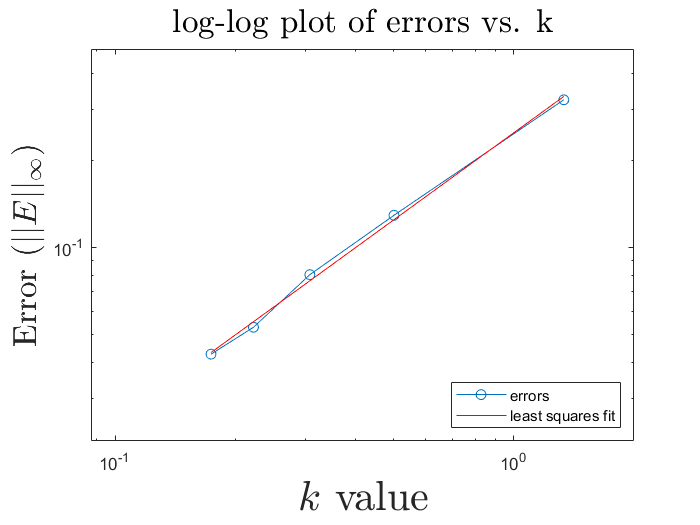
\includegraphics[scale = 0.4]{trbdf2errorkodd.png}
        \newline
        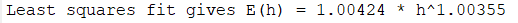
\includegraphics[scale = 0.6]{trbdf2orderh.PNG}
        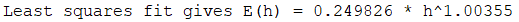
\includegraphics[scale = 0.6]{trbdf2orderk.PNG}
    \end{center}
\end{itemize}
Which turns out to be the same order that we find for the the Crank-Nicolson method (odd number of spacial points):
\begin{center}
    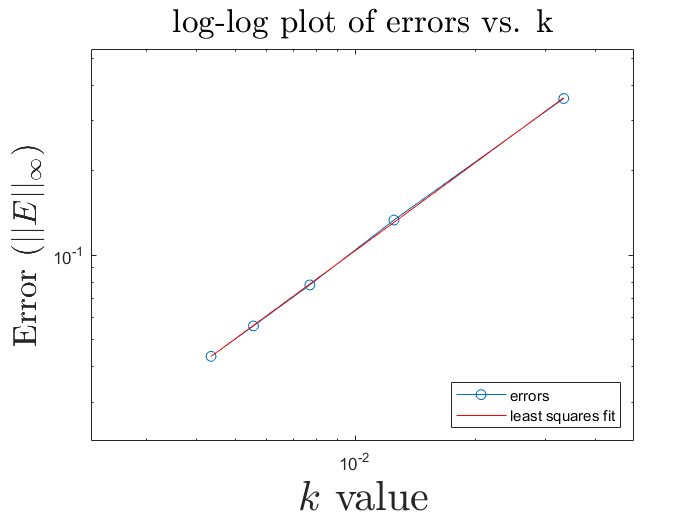
\includegraphics[scale = 0.4]{cnerrorkodd.png}
    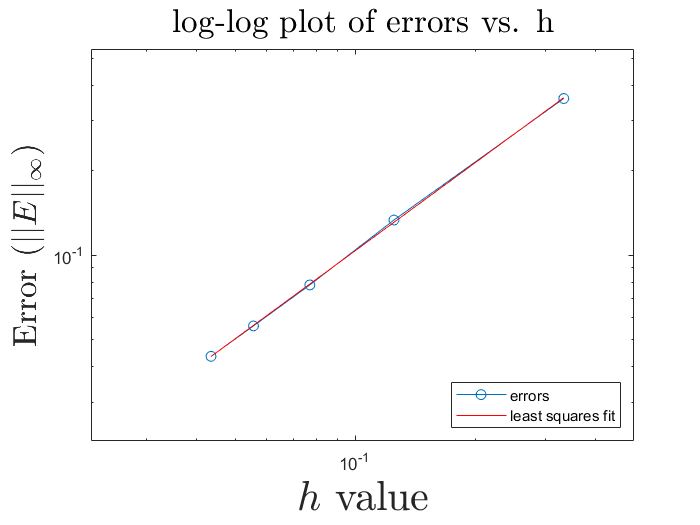
\includegraphics[scale = 0.4]{cnerrorhodd.png}
    \newline
    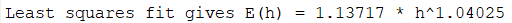
\includegraphics[scale = 0.6]{cnorderhodd.PNG}
    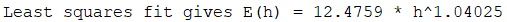
\includegraphics[scale = 0.6]{cnorderkodd.PNG}
\end{center}
\end{document}
